% -*- root: ../thesis.tex -*-
 \chapter{Modele uwzględniające istnienie kompleksów MAM}
 \label{chap:model}

W rozdziale tym przedstawione zostały całokomórkowe modele uwzględniające obecność mitochondrialnych magazynów wapniowych ze szczególnym uwzględnieniem obszarów ich bliskiego sąsiedztwa z retikulum endoplazmatycznym (Mitochondria Associated Membrane Complexes - Rozdz.~\ref{s:kompleksy_blonowe}). Modele te stanowią rozwinięcie prac \cite{Marhl2000,Schuster2002} wprowadzając dodatkowe przepływy retikulkarno-mitochondrialne oraz zmodyfikowane przepływy cytozoliczno-mitochondrialne.

\section{Opis modeli}

W niniejszym rozdziale przedstawione zostaną dwa modele ewolucji uśrednionego stężenia jonów wapnia w trój-kompartmentowym opisie komórki eukariotycznej (\textbf{cytozol}, \textbf{siateczka śródplazmatyczna} i \textbf{mitochondria}). Jak już wspominaliśmy, celem obydwu modeli jest uwzględnienie połączeń między siateczką śródplazmatyczną a~mitochondriami, których istnienie pozwala na prawie bezpośredni przepływ jonów wapnia pomiędzy tymi organellami \cite{Dyzma2012,Szopa2013}. W drugim modelu \cite{Szopa2013} zostały wzięte dodatkowo pod uwagę dwa tryby pracy białka transportującego wapń do wnętrza mitochondriów: tryb RaMowy (RaM - Rapid Uptake Mode) oraz tryb normalny (Rozdz.~\ref{ss:uniporter}).

\medskip

Ze względu na wspomnianą powyżej bezpośrednią bliskość retikulum endoplazmatycznego i mitochondriów, kompleksy MAM spełniają niezwykle ważną rolę w homeostazie i dynamice wapnia w komórce (Rozdz.~\ref{ss:MAM}). Ułatwiony przepływ wapnia pomiędzy powyższymi kompartmentami komórkowymi może wpływać istotnie np. na stany równowagowe wapnia oraz na oscylacje stężeń wolnych jonów wapnia w poszczególnych częściach komórki. Oscylacje takie są niezbędne do prawidłowego funkcjonowania komórki. Mogą być m.in. odpowiedzialne za szereg istotnych procesów fizjologicznych, takich jak kontrola cyklu komórkowego, skurcz mięśni szkieletowych, wzmocnienie synaptyczne. Stabilne oscylacje wapniowe stanowią również istotny czynnik będący częścią sieci sygnałowej, sprawdzający, czy komórka jest w dobrej kondycji i utrzymujący ją przy życiu. Cykliczne wahanie poziomu wapnia w mitochondriach (w modelach matematycznych odpowiada im stabilny cykl graniczny) powoduje aktywację dehydrogenaz poprzez allosteryczne związanie jonów Ca$^{2+}$ i wzrost produkcji ATP. Zatem z jednej strony lokalne w czasie i przestrzeni zmiany stężenia wolnego wapnia cytozolicznego są jednym ze sposobów przenoszenia informacji w~komórce i inicjacji szeregu ścieżek sygnałowych będących odpowiedzią na zmieniające się warunki zewnętrzne, z~drugiej zaś zbyt wysoka koncentracja wolnych jonów wapnia w cytozolu jest bardzo szkodliwa i~może doprowadzić do śmierci komórki. (Wiadomo np., że wapń jest jednym z kilku czynników zapoczątkowujących apoptozę – kontrolowaną śmierć komórki \cite{Giorgi2012a}). Zasadniczo badanie wpływu kompleksów MAM na dynamikę wapnia w komórce należałoby przeprowadzić na gruncie modelu przestrzennego opisywanego układem równań różniczkowych cząstkowych przy uwzględnieniu informacji dotyczących rozmieszczenia i rozmiarów zbiorników retikularnych i mitochondrialnych w komórce. Zadanie takie jest jednak bardzo skomplikowane, zarówno z teoretycznego, jak i numerycznego punktu widzenia. Co więcej, dla tego typu układów, ze skomplikowana geometrią, olbrzymia ilością podobszarów i nieliniowymi przepływami miedzy nimi, niezwykle trudno znaleźć (numerycznie) rozwiązanie opisujące oscylacje w~czasie (i przestrzeni).

W naszych rozważaniach zdecydowaliśmy się zatem na pozostanie w ramach tzw. modeli całokomórkowych (,,whole cell models'' \cite{Keener2009}), które abstrahują od przestrzennego rozkładu retikulum i~mitochondriów wewnątrz komórki i analizują jedynie zależność od czasu stężeń wolnego wapnia uśrednionych przestrzennie po odpowiedniej składowej kompartmentalnej (cytozolicznej, retikularnej i mitochondrialnej) przy założeniu dostatecznie szybkiej dyfuzji wapnia. W tym podejściu opis zmienności czasowej wapnia opisuje się układem nieliniowych równań różniczkowych zwyczajnych. Ponieważ dokonujemy przestrzennego uśrednienia stężenia (a nawet zakładamy przestrzenną jednorodność stężeń), istnienie kompleksów MAM uwzględniamy poprzez wprowadzenie dodatkowego bezpośredniego przepływu wapnia pomiędzy retikulum a mitochondriami. (W modelach całokomórkowych nie biorących pod uwagę istnienia obszarów MAM, przepływ pomiędzy tymi kompartmentami odbywa się pośrednio przez cytozol.) Kompleksy MAM stanowią jedynie około 6-7 procent powierzchni zewnętrznej błony mitochondrialnej. Mimo tego, ich obecność może istotnie wpływać na szybkość wymiany wolnych jonów wapnia pomiędzy powyższymi organellami, gdyż przeważająca część receptorów IP$_3$ oraz kanałów VDAC, odpowiedzialnych za przepływ wapnia z~retikulum endoplazmatycznego do mitochondrium znajduje się w ich rejonie \cite{Gunter2000}. 

\medskip 

Podsumowując, zgodnie z konwencją modeli całokomórkowych rozważamy sytuację, w której rozmieszczenie jonów Ca$^{2+}$ jest przestrzennie jednorodne w każdym z rozpatrywanych przedziałów, może natomiast zmieniać się w czasie. Jony wapnia mogą przepływać pomiędzy trzema kompartmentami: siateczką śródplazmatyczną, mitochondriami i cytozolem. Wiązane są również przez białka buforujące obecne w każdym z wymienionych kompartmentów. Istnienie mikrodomen uwzględniamy poprzez wprowadzenie dodatkowego przepływu jonów wapnia pomiędzy ER i mitochondriami (Ryc.~\ref{fig:scheme}). 

Przedstawione modele zadane są układami równań różniczkowych zwyczajnych, opisujących zmiany stężenia wolnego i zbuforowanego wapnia w poszczególnych kompartmentach komórki. Modele te są modelami zamkniętymi - zakładamy, że wymiana wapnia cytozolicznego z macierzą pozakomórkową odbywa się na tyle wolno, że można ją zaniedbać w rozpatrywanej przez nas skali czasu. Założenie to jest uzasadnione, ponieważ w normalnych warunkach wymiana jonów wapnia między komórką a przestrzenią międzykomórkową jest o wiele wolniejsza, niż procesy przepływu wapnia pomiędzy kompartmentami wewnątrzkomórkowymi \cite{Sneyd2004}. Dodatkowo, zgodnie z \cite{Sneyd2004}, możliwe są ,,prawidłowe'' oscylacje wapniowe nawet w przypadku całkowitego zablokowania transportu wapnia przez błonę komórkową.


Jak zwykle, w przypadku stosowania modeli całokomórkowych, pojawia się pytanie o zasadność pominięcia efektów przestrzennych. Dla stosunkowo małych komórek (o~średnicy nieprzekraczającej 6 $\mu m$) dyfuzyjne wyrównywanie stężeń zachodzi na tyle szybko, iż można się spodziewać, że niejednorodności przestrzenne stężenia wapnia nie wpływają zarówno na istnienie, jak i na okres oscylacji. Szybkość dyfuzyjnego wyrównywania się stężenia wapnia można oszacować w przybliżeniu korzystając z klasycznego wzoru na zależność średniego kwadratu odległości, jaką cząstka Brownowska pokonuje w czasie $\Delta t$: 

\medskip
\begin{equation}\label{eq:dystans}
R^2=D_{\textit{eff}} \cdot \Delta t, 
\end{equation}
\medskip

\noindent gdzie $D_{\textit{eff}}$ oznacza efektywny współczynnik dyfuzji dla wapnia w obecności buforów (tj. biorący pod uwagę procesy odłączania i przyłączania jonów wapnia do molekuł buforujących). Współczynnik ten trudno oszacować analitycznie, głównie ze względu na dużą różnorodność molekuł buforujących o nieznanych parametrach $k_{-},k_+$ oraz współczynnikach dyfuzji. Jeśli jednak ograniczyć się do jednego reprezentatywnego rodzaju buforów oraz założyć, że $k_{-},k_+$ są relatywnie duże, to można podać przybliżony wzór na $D_{\textit{eff}}$. Wielkość $D_{\textit{eff}}$ nie jest stałą, zależy od stężeń wolnego wapnia, jak i stężenia wapnia zbuforowanego (por. równania (7.76) oraz (7.77) w książce \cite{Keener2009}). Dla charakterystycznych buforów endogennych można oszacować $D_{\textit{eff}} \cong 20-30 \, \mu m^2/s$, co jest wielkością o rząd mniejszą niż współczynnik dyfuzji wapnia w cytozolu wynoszący około $300 \mu m^2/s$. Przyjmując zatem $D_{\textit{eff}} = 20 \mu m^2/s$ wnioskujemy, że jony wapniowe przesuną się średnio na odległość równą $6 \mu m$ po czasie $\Delta t \cong 1.68\,s$, co stanowi około 1/10 okresu znalezionych oscylacji. Dla stosunkowo małych komórek założenie jednorodności przestrzennej stężeń jonów wapnia w cytozolu (i innych kompartmentach) jest zatem dość dobrze usprawiedliwione. Dla większych komórek założenie to może być poddane w wątpliwość, jest jednak bardzo często stosowane. Należy bowiem wziąć pod uwagę fakt, że oscylacje wapniowe mogą mieć charakter quasi-lokalny, tzn. mogą odbywać się prawie niezależnie w pewnych dostatecznie małych podobszarach komórki. 

Innym problemem pojawiającym się przy próbach stosowania modeli opartych na deterministycznych równaniach różniczkowych zwyczajnych jest stochastyczna natura aktywności pojedynczych kanałów wapniowych, która przybiera formę nieregularnych w czasie wydarzeń polegających na ich otwieraniu i zamykaniu. (Otwarcie kanału połączone z wypływem wapnia na zewnątrz zbiornika w języku angielskim nosi nazwę ,,blip''.) Takie pojedyncze otwarcie może generować stochastyczne pobudzenie całego pojedynczego klastra kanałów \cite{Skupin2010}. (Wypływ wapnia z klastra kanałów w języku angielskim określany jest mianem ,,puff''.) Opis deterministyczny nieprzestrzenny może być jednak usprawiedliwiony z uwagi na fakt, że wypływy wapnia z poszczególnych klastrów mogą zachodzić w sposób zsynchronizowany, jeśli są wynikiem dostatecznie silnej stymulacji zewnętrznej. Taka sytuacja ma miejsce nawet w dużych komórkach, takich jak hepatocyty \cite{Dupont2009}.

\FloatBarrier
\subsection{Model \#1}
\label{ss:Mo1}

Punktem wyjścia do budowy pierwszego modelu (zwanego dalej \textbf{Modelem \#1}) był model zaproponowany przez Marhla i współpracowników z roku 2000~\cite{Marhl2000} oraz \cite{Schuster2002}. Jest to jeden z nielicznych modeli, który uwzględnia aktywny wpływ mitochondriów na dynamikę sygnału wapniowego w komórce i nie traktuje ich jedynie jak olbrzymich cząsteczek buforujących. W~Modelu \#1, wymiana wapnia pomiędzy ER a~mitochondrium odbywa się poprzez cytozol oraz bezpośrednio z magazynów retikularnych do mitochondriów w miejscach ich bliskiego kontaktu, tzn. wewnątrz obszarów MAM. Prędkość przepływu jonów wapnia w tych obszarach oznaczana symbolem $J_{MAM}$ (Ryc.~\ref{fig:scheme}), zależy od stężenia jonów wapnia w miejscach uwalniania ich ze światła retikulum endoplazmatycznego. Stężenie to jest porównywalne ze stężeniem tych jonów wewnątrz retikulum ($[Ca^{2+}]_{ER}$) i średnio rzecz biorąc wyższe niż stężenie jonów wapnia w cytozolu ($[Ca^{2+}]_{Cyt}$) \cite{Dyzma2012}.

\begin{figure}[tb]
\centering
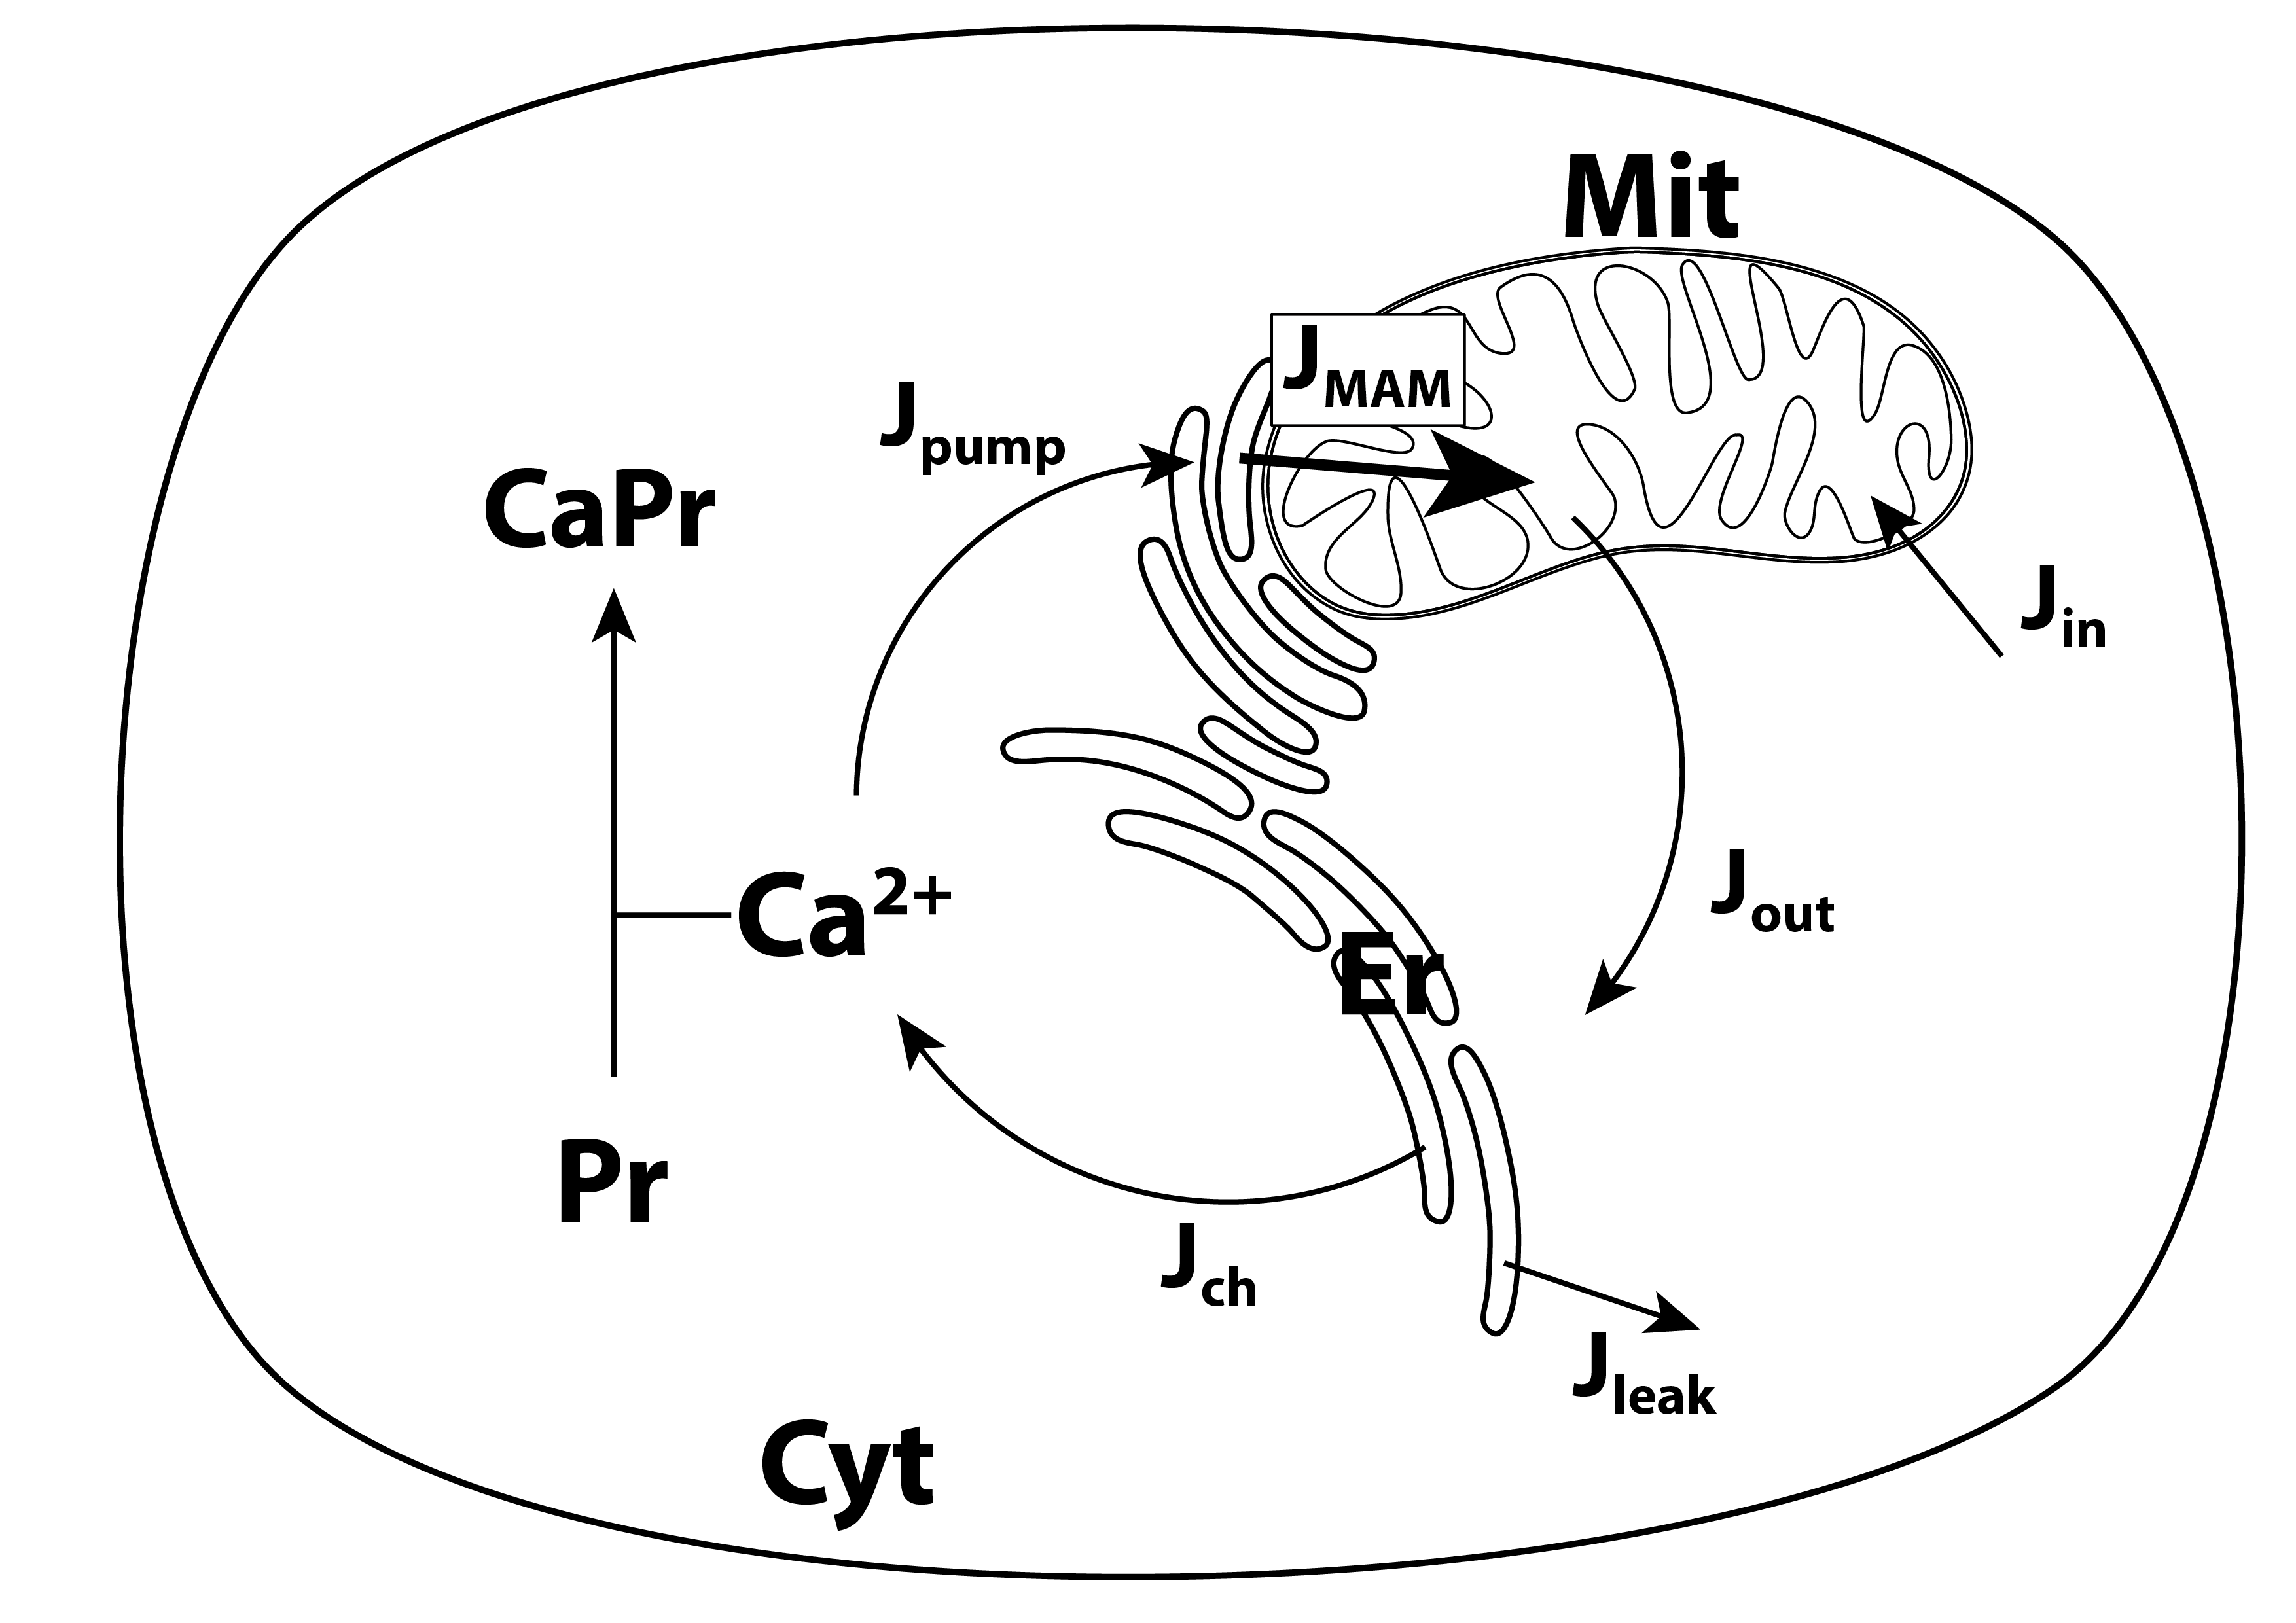
\includegraphics[width=0.8\textwidth]{rysunki/rozdzial_4/scheme.png}
\caption[Schematyczna reprezentacja modelu]{Schematyczna reprezentacja przepływów rozpatrzonych w modelach: \textbf{ER} -- siateczka śródplazmatyczna, \textbf{Mit} -- mitochondrium, \textbf{Cyt} -- cytozol; \textbf{CaPr} -- wapń zbuforowany; ${\boldsymbol J_{pump}}$ -- przepływ wapnia przez pompę w błonie retikulum; ${\boldsymbol J_{MAM}}$ -- bezpośredni przepływ z retikulum do mitochondrium; ${\boldsymbol J_{in}}$ -- pobieranie wapnia prze mitochondrium poprzez VDAC-MCU; ${\boldsymbol J_{out}}$ -- wypływ jonów wapnia z~mitochondrium przez wymiennik NCX; ${\boldsymbol J_{ch}}$ - wypływ jonów wapnia z ER; ${\boldsymbol J_{leak}}$ -- niespecyficzny wypływ z ER przez błony białkowo-lipidowe.}
\label{fig:scheme}
\end{figure}

Jak wspomniano w Rozdz.~\ref{s:kompleksy_blonowe} koncepcja istnienia wyizolowanych przestrzeni wewnątrz cytozolu, w których stężenie jonów wapniowych przewyższa znacznie stężenie jonów wapniowych w innych obszarach cytozolu, pojawiła się już w latach 80. XX-go wieku \cite{Rizzuto2006} i była naturalnym wnioskiem z prac eksperymentalnych \cite{Ashby2002,Bezzi1998,Petersen1995,Poenie1987}. Nie została ona jednak uwzględniona \textit{explicite} w żadnym z dotychczasowych całokomórkowych modeli opisujących ewolucję wapnia w komórce eukariotycznej. Uwzględnienie tego typu obszarów jest właśnie przedmiotem modyfikacji modelu Marhla, których efektem są zapropoponowane przez nas modele: Model \#1 oraz Model \#2. Wprowadzenie bezpośredniego przepływu jonów wapnia $J_{MAM}$ nie wynika \textit{jedynie} z faktu niemożności odzwierciedlenia bliskości struktur retikularnych i mitochondrialnych w~modelu nieprze-strzennym, ale ma również \textit{istotne usprawiedliwienie biologiczne} wynikające z~istnienia mikrodomen typu MAM. Ten specyficzny interfejs, który tworzy się pomiędzy retikulum i mitochondriami jest w znacznej mierze przestrzenią odizolowaną od pozostałej części cytozolu. Specyficzne białka stabilizujące apozycje błon mitochondrium-ER (np. mitofuzyna-2, lub grp75) ograniczają przestrzeń pomiędzy błonami formując swoisty ,,tunel'' dla jonów wapnia. We wcześniejszych pracach autorzy sugerowali wprawdzie istnienie mikrodomen, ale jedynie poprzez zmniejszanie stałej półaktywacji dla uniportera mitochondrialnego \cite{Marhl2000,Marhl1998}. Zaproponowane przez nas modele pozwalają również na rozróżnienie dwóch populacji białek transportujących wapń do mitochondrium. Jedna - związana z ,,obszarem MAM'' eksponowana jest na stężenie Ca$^{2+}$ obecne w retikulum endoplazmatycznym, druga na stężenie jonów wapnia w~cytozolu.


\par{\textbf{Układ równań różniczkowych zwyczajnych opisujący Model \#1}} 

Stężenie wolnych jonów wapnia w cytozolu ($Ca_{Cyt}$), retikulum endoplazmatycznym ($Ca_{ER}$) i mitochondriach ($Ca_{Mit}$), stężenie ,,uwapniowanych'' miejsc wiązania $CaPr$ w~cytozolu oraz stężenie miejsc wiązania cytozolicznych białek buforujących ($Pr$) w~czasie opisują równania:

\flushbottom

\begin{align}
\frac{dCa_{Cyt}}{dt}&=J_{ch}+J_{leak}-J_{pump}+J_{out}-J_{in} \label{eq:1} 
			+k_-CaPr-k_+Ca_{Cyt}Pr, \\
\frac{dCa_{ER}}{dt}&=\frac{\beta_{ER}}{\rho_{ER}}\left(J_{pump}-J_{ch}
			-J_{leak} -J_{MAM}\right), \label{eq:2}\\
\frac{dCa_{Mit}}{dt}&=\frac{\beta_{Mit}}{\rho_{Mit}}\left(J_{in}+J_{MAM}
			-J_{out}\right), \label{eq:3}\\
\frac{dCaPr}{dt}&= k_+ Ca_{Cyt}Pr - k_-CaPr, \label{eq:4}\\
\frac{dPr}{dt}&= -k_+ Ca_{Cyt}Pr + k_-CaPr. \label{eq:5}
\end{align}


\medskip 

\noindent W powyższych równaniach $\rho_i$ oznacza objętościowy współczynnik skalujący dla $i$-tego kompartmentu, $i \in \{ER, Mit\}$. 	Tak więc

	\begin{equation} \label{rhoi}
	\rho_i = \dfrac{V_{i}}{V_{Cyt}}
	\end{equation}
	
\noindent gdzie $V_i$ oznacza objętość $i$-tego kompartmentu. $\beta_i$ oznacza stosunek stężeń wolnych jonów wapnia do stężenia całkowitego wapnia w $i$-tym kompartmencie, $i \in \{ER, Mit\}$. Tak więc 
	
	\begin{equation} \label{beta_i} 
	\beta_i = \dfrac{Ca_{i}}{Ca_i + Ca_iPr}
	\end{equation}
	
\noindent gdzie $Ca_iPr$ - stężenie uwapniowanych miejsc wiązania buforów w $i$-tym kompartmencie (por. Rozdz.~\ref{ch:bufory}). 
		
\medskip 

Dodając równania (\ref{eq:1})-(\ref{eq:5}) otrzymujemy zależność: 


\begin{equation} \label{eq:cons:Ca}
Ca_{Cyt}(t) + \frac{\rho_{ER}}{\beta_{ER}}Ca_{ER}(t) 
+ \frac{\rho_{Mit}}{\beta_{Mit}}Ca_{Mit}(t) + CaPr(t) = const:=Ca_{tot} 
\end{equation}

\noindent Równanie to wyraża prawo zachowania całkowitej ilości wapnia w~układzie. Możemy się o tym przekonać mnożąc je przez objętość cytozolu $V_{Cyt}$. Otrzymujemy bowiem wtedy równanie: 

\begin{equation} \label{eq:cons:CaV}
\begin{array}{l}
V_{Cyt}Ca_{Cyt}(t) + V_{Cyt} CaPr(t) + \\[3ex] 
V_{ER} \frac{1}{\beta_{ER}}Ca_{ER}(t) 
+ V_{Mit} \frac{1}{\beta_{Mit}}Ca_{Mit}(t) = 
V_{Cyt} Ca_{tot} = const, 
\end{array}
\end{equation}

\noindent w którym lewa strona w sposób oczywisty przedstawia sumę całkowitej ilości jonów wapniowych w poszczególnych kompartmentach. 


Dodając równania (\ref{eq:4}) i (\ref{eq:5}) otrzymujemy $\dfrac{d}{dt} (CaPr + Pr) = 0$, co pozostaje w~zgodzie z faktem, że całkowite stężenie miejsc wiązania jonów wapnia przez bufory (tj. miejsc ze związanymi jonami wapnia oraz miejsc niezwiązanych) $Pr_{tot}$ jest stałe w~czasie: 
 
\begin{equation} \label{eq:cons:Pr}
Pr_{tot}(t) := Pr(t) + CaPr(t) = Pr(0) + CaPr(0)=:Pr_{tot}.
\end{equation}

\noindent Tak więc, dzięki prawom zachowania (\ref{eq:cons:Ca}) i (\ref{eq:cons:Pr}) układ równań (\ref{eq:1})--(\ref{eq:5}) może zostać zredukowany do układu trzech równań różniczkowych zwyczajnych:

\begin{eqnarray}\nonumber
\frac{dCa_{Cyt}}{dt}&=&J_{ch}+J_{leak}-J_{pump}+J_{out}-J_{in}\\
			&& +k_-CaPr-k_+Ca_{Cyt}(Pr_{tot} - CaPr), \label{eq:1a}\\
\frac{dCa_{ER}}{dt}&=&\frac{\beta_{ER}}{\rho_{ER}}\left(J_{pump}-J_{ch}
			-J_{leak} -J_{MAM}\right), \label{eq:2a}\\
\frac{dCa_{Mit}}{dt}&=&\frac{\beta_{Mit}}{\rho_{Mit}}\left(J_{in}+J_{MAM}
			-J_{out}\right). \label{eq:3a}
\end{eqnarray}

\noindent gdzie ilość wapnia związanego przez bufory możemy wyliczyć ze wzoru (\ref{eq:cons:Ca}):

\begin{equation} \label{eq:CaPr}
CaPr = Ca_{tot} - Ca_{Cyt} - \frac{\rho_{ER}}{\beta_{ER}}Ca_{ER} 
				- \frac{\rho_{Mit}}{\beta_{Mit}}Ca_{Mit}.
\end{equation}

Poszczególne przepływy realizowane przez pompy, kanały wapniowe i wymienniki opisane są poprzez prądy wapniowe $J_{()}$. Aktywny transport jonów Ca$^{2+}$ do światła retikulum endoplazmatycznego $J_{pump}$ realizowany jest przez białka SERCA, natomiast wypływ jonów wapnia z ER realizowany jest przez kanały wapniowe IP$_3$R/RyR (przepływ $J_{ch}$) oraz niespecyficzny wypływ $J_{leak}$. Przepływy te opisywane są wyrażeniami:

\begin{align}
J_{pump}&= k_{pump}Ca_{Cyt},\\
J_{ch}&= k_{ch}\frac{Ca_{Cyt}^2}{K_1^2+Ca_{Cyt}^2}
											\left(Ca_{ER}-Ca_{Cyt}\right),\label{eq:Jch}\\
J_{leak}&= k_{leak}\left(Ca_{ER}-Ca_{Cyt}\right).
\end{align}

$J_{pump}$ zależy bezpośrednio od stężenia Ca$^{2+}$ w cytozolu. Stała $k_{pump}$ określa tempo przepływu. Wypływ jonów wapnia z ER zależy od gradientu jonów wapnia pomiędzy cytozolem, a światłem ER ($Ca_{ER}-Ca_{Cyt}$). Stała $k_{ch}$ określa maksymalną przepuszczalność kanału wapniowego, natomiast $K_1$ jest stałą półaktywacji. Funkcja Hilla w~wyrażeniu $J_{ch}$~(\ref{eq:Jch}) opisje mechanizm CICR. Niespecyficzny wypływ jonów wapnia ($J_{leak}$) zależy od różnicy stężeń jonów wapnia w~poprzek błony retikulum, $k_{leak}$ określa tempo wypływu jonów wapnia z ER.

Dynamika wapnia w mitochondrium zadana jest następującymi przepływami:

\begin{align}
J_{MAM}&= k_{MAM} \frac{Ca_{ER}^8}{K_4^8 + Ca_{ER}^8},\label{eq:jmamMo1}\\
J_{in}&= k_{in2}\frac{Ca_{Cyt}^8}{K_2^8+Ca_{Cyt}^8},\label{eq:jinMo1}\\
J_{out}&= \left(k_{out}\frac{Ca_{Cyt}^2}{K_3^2+Ca_{Cyt}^2}+k_m\right)
Ca_{Mit}.\label{eq:joutMo1}
\end{align}

$J_{MAM}$ opisuje bezpośredni przepływ jonów wapnia z ER do mitochondriów, implikowany faktem istnienia mikrodomen MAM. Stała $k_{MAM}$ określa maksymalną przepustowość interfejsu MAM, a $K_4$ stałą półaktywacji. Z drugiej strony, $J_{in}$ opisuje napływ jonów wapnia do mitochondrium przez białka transportowe położone poza obszarami MAM. Powolny wypływ jonów wapnia z mitochondrium odbywa się poprzez wymienniki \mbox{Na$^+$/Ca$^{2+}$} (NCX) i \mbox{H$^+$/Ca$^{2+}$} (HCX). Ze względu na to, że przepływ ten ma jedynie nieznaczny wpływ na potencjał transbłonowy mitochondrium $\Delta \Psi_m$ (\cite{Babcock1997}, Rozdz.~3.4 w \cite{Falcke2004}), zmiany $\Delta \Psi_m$ w powyższym modelu zostały pominięte. Całkowity przepływ jonów wapnia z mitochondrium do cytozolu określa zatem wyrażenie $J_{out}$, w którym $k_m$ jest stałą określającą wypływ niespecyficzny, a $k_{out}$ oznacza maksymalny przepływ jonów wapnia przez wymienniki NCX/HCX. $K_3$
jest stałą półaktywacji.

\FloatBarrier
\subsection{Model \#2}
Układ równań różniczkowych zwyczajnych opisujący zmiany stężenia wolnych jonów wapnia w Modelu \#2, jest tożsamy z układem (\ref{eq:1})-(\ref{eq:5}). Różnice dotyczą jedynie konkretnych postaci funkcji $J_{MAM}$ (wyrażenia (\ref{eq:jmamMo1}) i~(\ref{eq:jmamMo2})), $J_{in}$ (wyrażenia (\ref{eq:jinMo1}) i~(\ref{eq:jinMo2})) oraz $J_{out}$ (wyrażenia (\ref{eq:joutMo1}) i (\ref{eq:joutMo2})). Rozpatrywany układ ma zatem postać:

\begin{align}
\frac{dCa_{Cyt}}{dt}&=J_{ch}+J_{leak}-J_{pump}+J_{out}-J_{in} \label{eq:1aa} 
			+k_-CaPr-k_+Ca_{Cyt}Pr, \\
\frac{dCa_{ER}}{dt}&=\frac{\beta_{ER}}{\rho_{ER}}\left(J_{pump}-J_{ch}
			-J_{leak} -J_{MAM}\right), \label{eq:2aa}\\
\frac{dCa_{Mit}}{dt}&=\frac{\beta_{Mit}}{\rho_{Mit}}\left(J_{in}+J_{MAM}
			-J_{out}\right), \label{eq:3aa}\\
\frac{dCaPr}{dt}&= k_+ Ca_{Cyt}Pr - k_-CaPr, \label{eq:4aa}\\
\frac{dPr}{dt}&= -k_+ Ca_{Cyt}Pr + k_-CaPr. \label{eq:5aa}
\end{align} 


Jak w przypadku Modelu \#1 słuszne są prawa zachowania 
(\ref{eq:cons:Ca}) oraz (\ref{eq:cons:Pr}). 
W~konsekwencji układ (\ref{eq:1aa})-(\ref{eq:5aa}) można zredukować 
do trzech równań postaci (\ref{eq:1a})-(\ref{eq:3a}): 

\begin{align}
\frac{dCa_{Cyt}}{dt}&=J_{ch}+J_{leak}-J_{pump}+J_{out}-J_{in}
			+k_-CaPr-k_+Ca_{Cyt}Pr, \label{eq:11}\\
\frac{dCa_{ER}}{dt}&=\frac{\beta_{ER}}{\rho_{ER}}\left(J_{pump}-J_{ch}
			-J_{leak} -J_{MAM}\right), \label{eq:22}\\
\frac{dCa_{Mit}}{dt}&=\frac{\beta_{Mit}}{\rho_{Mit}}\left(J_{in}+J_{MAM}
			-J_{out}\right). \label{eq:33}
\end{align}



Przepływy retikularno-cytozoliczne: $J_{pump}$ (aktywność pompy retikularnej), $J_{ch}$~(wypływ poprzez kanały wapniowe IP$_3$R/RyR) oraz $J_{leak}$ (niespecyficzny przepływ Ca$^{2+}$ przez błony biologiczne) dane są jak w przypadku Modelu \#1 następującymi wyrażeniami:

\begin{align}
J_{pump}& = k_{pump}Ca_{Cyt},\\
J_{ch}& = k_{ch}\frac{Ca_{Cyt}^2}{K_1^2+Ca_{Cyt}^2}
											\left(Ca_{ER}-Ca_{Cyt}\right),\label{eq:jch}\\
J_{leak}& = k_{leak}\left(Ca_{ER}-Ca_{Cyt}\right).
\end{align}


\subsubsection*{Różnice pomiędzy Modelem~\#2 i Modelem~\#1}
\label{ss:roznice}

W Modelu~\#2 uwzględniono nie tylko aktywny udział mitochondriów, ale również właściwości białka transportującego wapń do wnętrza mitochondrium – uniportera mitochondrialnego (MICU). Uniporter w warunkach ekspozycji na nanomolowe (do 200 nM) stężenia wapnia aktywuje tzw. szybki mechanizm pobierania jonów wapniowych RaM (ang. rapid uptake mode). Doświadczenia przeprowadzone przez Vinogradova \cite{Vinogradov1973} oraz Guntera i współpracowników \cite{Gunter2001,Sparagna1995} sugerują, że w tych warunkach mitochondria pobierają wapń znacznie wydajniej. Przepływ do mitochondrium składa się zatem z~dwóch części. Pierwsza z nich uwzględnia wspomniany powyżej szybki tryb RaM-owy, druga opisuje pracę uniportera mitochondrialnego w trybie standardowym. Rozróżnienie takie odzwierciedla się w wyrażeniach na prądy $J_{MAM}$ oraz $J_{in}$ opisujące odpowiednio wpływ jonów wapnia do mitochondriów w obszarze interfejsu MAM oraz na pozostałej wewnętrznej powierzchni mitochondriów. Tak więc w Modelu \#2 wyrażenia na $J_{MAM}$ i $J_{in}$ mają postać:

\begin{align}
	J_{MAM} &= J_{MAM2} + J_{MAM8} := k_{MAM2} \frac{Ca_{ER}^2}{K_{4,2}^2 + Ca_{ER}^2}% \\[3ex]
	+ k_{MAM8} \frac{Ca_{ER}^8}{K_{4,8}^8 + Ca_{ER}^8},\label{eq:jmamMo2}\\
J_{in} &= J_{in2} + J_{in8}:=k_{in2}\frac{Ca_{Cyt}^2}{K_{2,2}^2+Ca_{Cyt}^2} 
				+ k_{in8}\frac{Ca_{Cyt}^8}{K_{2,8}^8+Ca_{Cyt}^8}.\label{eq:jinMo2}
\end{align}

W przeciwieństwie do Modelu~\#1, w Modelu~\#2 nie uwzględniono wpływu stężenia jonów wapnia w cytozolu na jego wypływ z mitochondriów poprzez czynnik 

\[k_{out}\frac{Ca_{Cyt}^2}{K_3^2+Ca_{Cyt}^2}\cdot Ca_{Mit}\]

Z drugiej strony zamiast liniowej proporcjonalności wypływu do $Ca_{Mit}$ przepływ ten modelowany jest za pomocą funkcji Hilla pierwszego rzędu. Zatem:

\begin{equation}
J_{out} = k_{out}\frac{Ca_{Mit}}{K_3+Ca_{Mit}} \label{eq:joutMo2}
\end{equation}

\noindent gdzie pominęliśmy dodatkowo niespecyficzny wypływ wapnia z mitochondrium \\$k_{m}\cdot Ca_{Mit}$.

Zmiana wyrażenia na $J_{out}$ w stosunku do Modelu~\#1 implikuje znaczące różnice w~jakościowym zachowaniu się układu. Najważniejszym przejawem różnic jest niewystępowanie rozwiązań chaotycznych, występujących dla odpowiedniego zestawu parametrów w Modelu~\#1.

\FloatBarrier
\section{Parametry i skalowanie}\label{sec:parametry}

W przypadku obu modeli przyjęliśmy wartość parametru Ca$_{tot}$ = 90 $\mu$M. Jak widać z postaci równań na ewolucję stężeń jonów wapnia w kompartmentach retikularnym i~mitochondrialnym, zależą one jedynie od stosunków $\frac{\beta_{ER}}{\rho_{ER}}$ oraz $\frac{\beta_{Mit}}{\rho_{Mit}}$ a nie od konkretnych wartości współczynników $\beta$ i $\rho$. Z tego też powodu w pracach \cite{Dyzma2012} oraz \cite{Szopa2013} wartości tych współczynników mają przypisane wartości zgodne z pracą \cite{Marhl2000}, ponieważ istotny jest jedynie stosunek obu wartości. Współczynniki $\beta_{ER}$ oraz $\beta_{Mit}$ są określone jedynie w przybliżeniu, chociaż uważa się, że ich fizjologiczne wartości powinny być mniejsze niż ok. 0.05. Z drugiej strony wartości współczynników $\rho$ są stosunkowo dobrze określone, chociaż zależą od rodzaju komórek. Dla większości komórek $\rho_{ER}$ oraz $\rho_{Mit}$ są rzędu około 0.1 (chociaż w pracy Marhla \cite{Marhl2000} współczynniki te zostały wybrane jako 0.01). Ustalając wartości stosunków $\frac{\beta_{ER}}{\rho_{ER}}=1/4$ oraz $\frac{\beta_{Mit}}{\rho_{Mit}}=1/4$ zapewniające występowanie oscylacji w rozpatrywanym układzie, otrzymujemy przybliżone wartości współczynników $\beta$ równe w przybliżeniu 0.025. 

\medskip 

Parametry kinetyczne określają maksymalne przepływy jonów wapnia przez dany transporter. Nazwy stałych pochodzą od nazw własnych poszczególnych przepływów. Wartości te (przedstawione małymi literami) oparte są na danych eksperymentalnych \cite{Marhl2000}. Dużymi literami przedstawione zostały z kolei stale półaktywacji poszczególnych białek transportujących wapń. Wszystkie parametry zgromadzone zostały w Tab.~\ref{tab:constantsMo1} oraz Tab.~\ref{tab:constantsMo2}.

\bigskip

\begin{table}[!ht]
	\centering
	\begin{tabular} {@{} l l l l l l @{}}
		\toprule[0.12em]
		Parametr 						& \multicolumn{2}{c}{Wartość} 	& Parametr			&\multicolumn{2}{c}{Wartość}			\\ \midrule[0.06em]
		\textit{Stężenia} 			&			& 			& \textit{Parametry kinetyczne}	& 			& 						\\
		$\textrm{Ca}_{tot}$				&	90		& $\mu$M	& $k_{ch}$					& 4100		& s$^{-1}$ 				\\
		$\textrm{Pr}_{tot}$				&	120		& $\mu$M	& $k_{pump}$				& 20 		& s$^{-1}$ 				\\
		&			&			& $k_{leak}$				& 0.05		& s$^{-1}$ 				\\
		\textit{Stałe objętościowe}			&			&			& $k_{in}$					& 300		& $\mu$Ms$^{-1}$		\\
		$\rho_{ER}$						&	0.01 	&			& $k_{out}$					& 125 		& s$^{-1}$ 				\\
		$\rho_{Mit}$					&	0.01	&			& $k_{MAM}$					& 1200		& $\mu$Ms$^{-1}$		\\
		&			&			& $k_{m}$					& 0.00625	& s$^{-1}$				\\
		\textit{Stałe buforujące}	&			&			& $k_{+}$					& 0.1		& $\mu$M$^{-1}$s$^{-1}$	\\
		$\beta_{ER}$					&	0.0025	&			& $k_{-}$					& 0.01		& $s^{-1}$				\\
		$\beta_{Mit}$					&	0.0025	&			& $K_{1}$					& 5			& $\mu$M				\\
		&			&			& $K_{2}$					& 0.8 		& $\mu$M				\\
		&			&			& $K_{3}$					& 5			& $\mu$M				\\
		&			&			& $K_{4}$					& 2.8		& $\mu$M				\\\bottomrule[0.12em]
	\end{tabular}
	\caption[Parametry użyte w Modelu \#1]{Parametry użyte w \textbf{Modelu \#1}.}
	\label{tab:constantsMo1}
\end{table}

\bigskip

\begin{table}[ht]
\centering
\begin{tabular} {@{} l r l l r l @{}}
\toprule[0.12em]
\rule{0pt}{3ex} \textbf{Parametr} 	& \multicolumn{2}{c}{\textbf{Wartość}} 	& \textbf{Parametr} &\multicolumn{2}{c}{\textbf{Wartość}} \\\midrule[0.06em]
\textit{Stężenia}	       	&	              	& 	    		& \textit{Wartości '$\beta/\rho$'}	&	   &	\\
$Ca_{tot}$							&	90	  	& $\mu$M				&	$\beta_{ER}(\rho_{ER})^{-1}$						&	0.25 &	\\
$Pr_{tot}$							&	120		& $\mu$M				&	$\beta_{Mit}(\rho_{Mit})^{-1}$						&	0.25 &	\\
									&			&						& 					&				&								\\
 \textit{Parametry kinetyczne} 	  &			& 		     		& \textit{Stałe półaktywacji}    & &		   \\
$k_{ch}$							& 4200		& s$^{-1}$ 				& $K_{1}$              & 5  & $\mu$M \\
$k_{pump}$							& 20 		& s$^{-1}$ 				& $K_{2,2}$             & 20 & $\mu$M \\
$k_{leak}$							& 0.05 	& s$^{-1}$ 				& $K_{2,8}$ 				    & 0.8 & $\mu$M \\
$k_{in2}$							& 20		& $\mu$Ms$^{-1}$		& $K_{3}$              & 3.1 & $\mu$M \\
$k_{in8}$							& 80 		& $\mu$Ms$^{-1}$		& $K_{4,2}$	            & 20 & $\mu$M \\
$k_{MAM2}$							& 50		& $\mu$Ms$^{-1}$		& $K_{4,8}$             & 1.8 & $\mu$M \\
$k_{MAM8}$							& 200		& $\mu$Ms$^{-1}$	  &                  &   &    \\
$k_{+}$								& 0.1		& $\mu$M$^{-1}$s$^{-1}$	& 					        &   &    \\
$k_{-}$								& 0.01 		& s$^{-1}$				&                  &   &    \\
$k_{out}$							& 1.9 		& $\mu$Ms$^{-1}$ 		& 					        &   &    \\
\bottomrule[0.12em]
\end{tabular}
\caption[Parametry użyte w Modelu \#2]{Parametry użyte w \textbf{Modelu \#2}.}
\label{tab:constantsMo2}
\end{table}



Dla większości symulacji wykonanych w ramach prac \cite{Dyzma2012} (Model \#1) oraz \cite{Szopa2013} (Model \#2) wykorzystywano zestawy parametrów przedstawione w tabelach \ref{tab:constantsMo1} oraz \ref{tab:constantsMo2}. Jeśli któryś z parametrów ulegał zmianie lub stawał się parametrem bifurkacyjnym było to wyraźnie zaznaczone.